% QMS Editor overview for management: agenda, design process, architecture, user guide, value. Gust SWI Template v3.
% Sheets: 1 agenda (1 hr 30 min review, in the pattern of the Open Orders team-review agenda), 2 design process,
% 3 system architecture, 4 user guide, 5 value to Doosan Bobcat. The agenda's miniatures follow sheets 2 to 5; keep in step.
% No pictures: every drawing is TikZ. Grid 12 x 7.5 in, scaled 4/3. Facts from the QMS Editor 2.0 architecture notes.
\documentclass[10pt]{article}
\usepackage[paperwidth=17in, paperheight=11in, margin=0.5in]{geometry}
\usepackage[T1]{fontenc}
\usepackage{lmodern}
\usepackage{microtype}
\usepackage{enumitem}
\usepackage{array}
\usepackage[table]{xcolor}
\usepackage{graphicx}
\usepackage{pifont}
\usepackage{tikz}
\usetikzlibrary{positioning, arrows.meta, calc, fit}
\usepackage[hidelinks, pdftitle={QMS Editor: Design, Architecture and Use}, pdfauthor={Gust F.}]{hyperref}
\pagestyle{empty}
\setlength{\parindent}{0pt}
\hyphenpenalty=10000
\exhyphenpenalty=10000
\setlist[itemize]{label=\textbullet, leftmargin=0.85em, labelsep=0.35em, itemsep=2.5pt, parsep=0pt,
                  topsep=0pt, partopsep=0pt}
\setlist[enumerate]{leftmargin=1.2em, labelsep=0.35em, itemsep=2.5pt, parsep=0pt, topsep=0pt, partopsep=0pt}
\definecolor{headgreen}{HTML}{548235}
\definecolor{bandgreen}{HTML}{E2EFDA}
\definecolor{flagpeach}{HTML}{FCE4D6}
\definecolor{inputyellow}{HTML}{FFFFCC}
\definecolor{alertorange}{HTML}{C55A11}
\tikzset{
  every node/.style={font=\sffamily\small, inner sep=5pt},
  box/.style={draw, line width=0.5pt, fill=white, align=left},
  station/.style={draw, line width=0.5pt, fill=headgreen, text=white, font=\sffamily\bfseries\normalsize,
                  align=left, inner ysep=4pt, text height=1.6ex, text depth=0.45ex},
  flow/.style={-{Stealth[length=9pt, width=6.5pt]}, line width=1.2pt, line join=miter},
  point/.style={-{Stealth[length=6pt, width=4.5pt]}, line width=0.9pt},
  marker/.style={circle, fill=headgreen, text=white, draw=white, line width=1pt, font=\sffamily\bfseries\small,
                 inner sep=0pt, minimum size=0.25in},
  shot/.style={draw, line width=0.5pt, inner sep=0pt, anchor=north west},
  layer/.style={draw=headgreen, line width=0.5pt, fill=bandgreen, align=left, anchor=north west},
  chip/.style={draw, line width=0.5pt, fill=white, align=center, font=\sffamily\footnotesize,
               minimum height=0.42in, inner sep=4pt},
  outchip/.style={chip, fill=bandgreen, font=\sffamily\bfseries\footnotesize},
}
\newcommand{\by}[1]{{\footnotesize\itshape #1\par}\vspace{5pt}}
\newcommand{\peach}[1]{{\setlength{\fboxsep}{1pt}\colorbox{flagpeach}{\textbf{#1}}}}
\newcommand{\btn}[1]{{\setlength{\fboxsep}{1.5pt}\fbox{\footnotesize\bfseries #1}}}
\newcommand{\num}[1]{\tikz[baseline=(n.base)]\node(n)[marker, minimum size=0.2in, font=\sffamily\bfseries\footnotesize]{#1};}
\newcommand{\val}[1]{{\ttfamily #1}}
% fixed-height box body, so the boxes in a row line up
\newcommand{\fixh}[2]{\begin{minipage}[t][#1][t]{\linewidth}#2\end{minipage}}
% big figure at the top of a box
\newcommand{\stat}[2]{{\color{headgreen}\bfseries\fontsize{26}{28}\selectfont #1}\\[2pt]{\footnotesize\itshape #2\par}\vspace{8pt}}
\newcommand{\badge}[1]{{\setlength{\fboxsep}{2pt}\colorbox{headgreen}{\textcolor{white}{\bfseries #1}}}}
% miniatures of sheets 2 to 5 for the agenda, drawn in each sheet's own 12 x 7.5 coordinates (use in a scaled scope)
\newcommand{\thumbframe}{%
  \draw[line width=0.5pt, fill=white] (0,0) rectangle (12,7.5);
  \fill (0.25,7.0) rectangle (3.4,7.25);
  \draw[line width=0.3pt] (5.7,0) -- (5.7,0.42) -- (12,0.42);}
\newcommand{\thumbbox}[4]{% x1, y top, x2, y bottom: a box with its green bar
  \draw[line width=0.3pt] (#1,#2) rectangle (#3,#4); \fill[headgreen] (#1,#2-0.3) rectangle (#3,#2);}
\newcommand{\thumbdesign}{%
  \thumbframe
  \foreach \a in {0.25, 2.61, 4.97, 7.33, 9.69} \thumbbox{\a}{6.4}{\a+2.06}{3.84};
  \thumbbox{0.25}{3.6}{7.39}{1.3} \thumbbox{7.75}{3.6}{11.75}{1.3}}
\newcommand{\thumbarch}{%
  \thumbframe
  \thumbbox{0.25}{6.4}{3.45}{2.75}
  \foreach \i in {0,...,4} \draw[line width=0.3pt, fill=bandgreen] (4.15,{6.02-0.6*\i}) rectangle (8.15,{5.5-0.6*\i});
  \fill[headgreen] (4.15,6.1) rectangle (8.15,6.4);
  \thumbbox{8.55}{6.4}{11.75}{2.98}
  \thumbbox{0.25}{2.6}{5.39}{0.6} \thumbbox{5.75}{2.6}{11.75}{0.6}}
\newcommand{\thumbguide}{%
  \thumbframe
  \foreach \a in {0.25, 2.61, 4.97, 7.33, 9.69} \thumbbox{\a}{6.4}{\a+2.06}{4.41};
  \thumbbox{0.25}{3.95}{6.94}{1.85} \thumbbox{7.36}{3.95}{11.75}{1.7}}
\newcommand{\thumbvalue}{%
  \thumbframe
  \foreach \a in {0.25, 4.2, 8.15} {\thumbbox{\a}{6.4}{\a+3.6}{3.81} \fill[headgreen] (\a+0.15,5.95) rectangle (\a+1.0,5.45);}
  \thumbbox{0.25}{3.45}{11.75}{1.71}}
% a document page with a folded corner, 0.56 x 0.72 in, anchored at its top left
\newcommand{\docicon}[2]{% x, y
  \draw[line width=0.5pt, fill=white] (#1,#2) -- (#1+0.42,#2) -- (#1+0.56,#2-0.14) -- (#1+0.56,#2-0.72) -- (#1,#2-0.72) -- cycle;
  \draw[line width=0.5pt] (#1+0.42,#2) -- (#1+0.42,#2-0.14) -- (#1+0.56,#2-0.14);
  \fill[headgreen] (#1+0.07,#2-0.08) rectangle (#1+0.36,#2-0.15);
  \draw[line width=0.5pt] (#1+0.28,#2-0.36) circle (0.08);
  \foreach \y in {0.54, 0.6} \draw[line width=0.4pt] (#1+0.07,#2-\y) -- (#1+0.49,#2-\y);}
% a layer of the app: bold name, technology on the right, role underneath
\newcommand{\layerbody}[3]{\textbf{#1}\hfill{\footnotesize\itshape #2}\\[2pt]{\footnotesize #3}}
\newcommand{\titleblock}[2]{%
  \draw[line width=0.5pt] (5.7,0) -- (5.7,0.42) -- (12,0.42);
  \foreach \x in {7.3, 8.95, 9.5, 9.95, 10.75, 11.45} \draw[line width=0.5pt] (\x,0) -- (\x,0.42);
  \foreach \x/\label/\value in {5.7/Title/#1, 7.3/Project/QMS Editor, 8.95/Version/2.0, 9.5/Rev./9,
                                9.95/Date/2026-10-22, 10.75/Drawn/Gust F., 11.45/Sheet/#2} {
    \node[anchor=north west, inner sep=0pt, font=\sffamily\fontsize{7}{8}\selectfont] at (\x+0.07,0.36) {\label};
    \node[anchor=south west, inner sep=0pt, font=\sffamily\bfseries\footnotesize] at (\x+0.07,0.07) {\value};
  }}
\newcommand{\heading}[2]{%
  \node[anchor=north west, inner sep=0pt, font=\sffamily\bfseries\fontsize{14}{16}\selectfont] at (0.25,7.25) {#1};
  \node[anchor=north west, inner sep=0pt, font=\sffamily\footnotesize] at (0.25,6.88) {#2};}
% the four sheets at the top right, the current one in green
\newcommand{\navitem}[3]{\ifnum#1=#2{\color{headgreen}\bfseries #3}\else #3\fi}
\newcommand{\nav}[1]{%
  \node[anchor=north east, inner sep=0pt, font=\sffamily\footnotesize] at (11.75,7.22)
    {\navitem{#1}{1}{1\enspace Agenda}\qquad\navitem{#1}{2}{2\enspace Design Process}\qquad
     \navitem{#1}{3}{3\enspace Architecture}\qquad\navitem{#1}{4}{4\enspace User Guide}\qquad
     \navitem{#1}{5}{5\enspace Value}};}

\begin{document}
% ================================================================ sheet 1: agenda
% timeline: 90 minutes from x = 0.5 to x = 11.5 (11/90 in a minute): 0:05 at 1.1111, 0:15 at 2.3333, 0:20 at 2.9444,
% 0:40 at 5.3889, 1:10 at 9.0556; QMS-001 to QMS-005 take 6 min (0.7333 in) each from 0:40
\noindent\scalebox{1.333333}{%
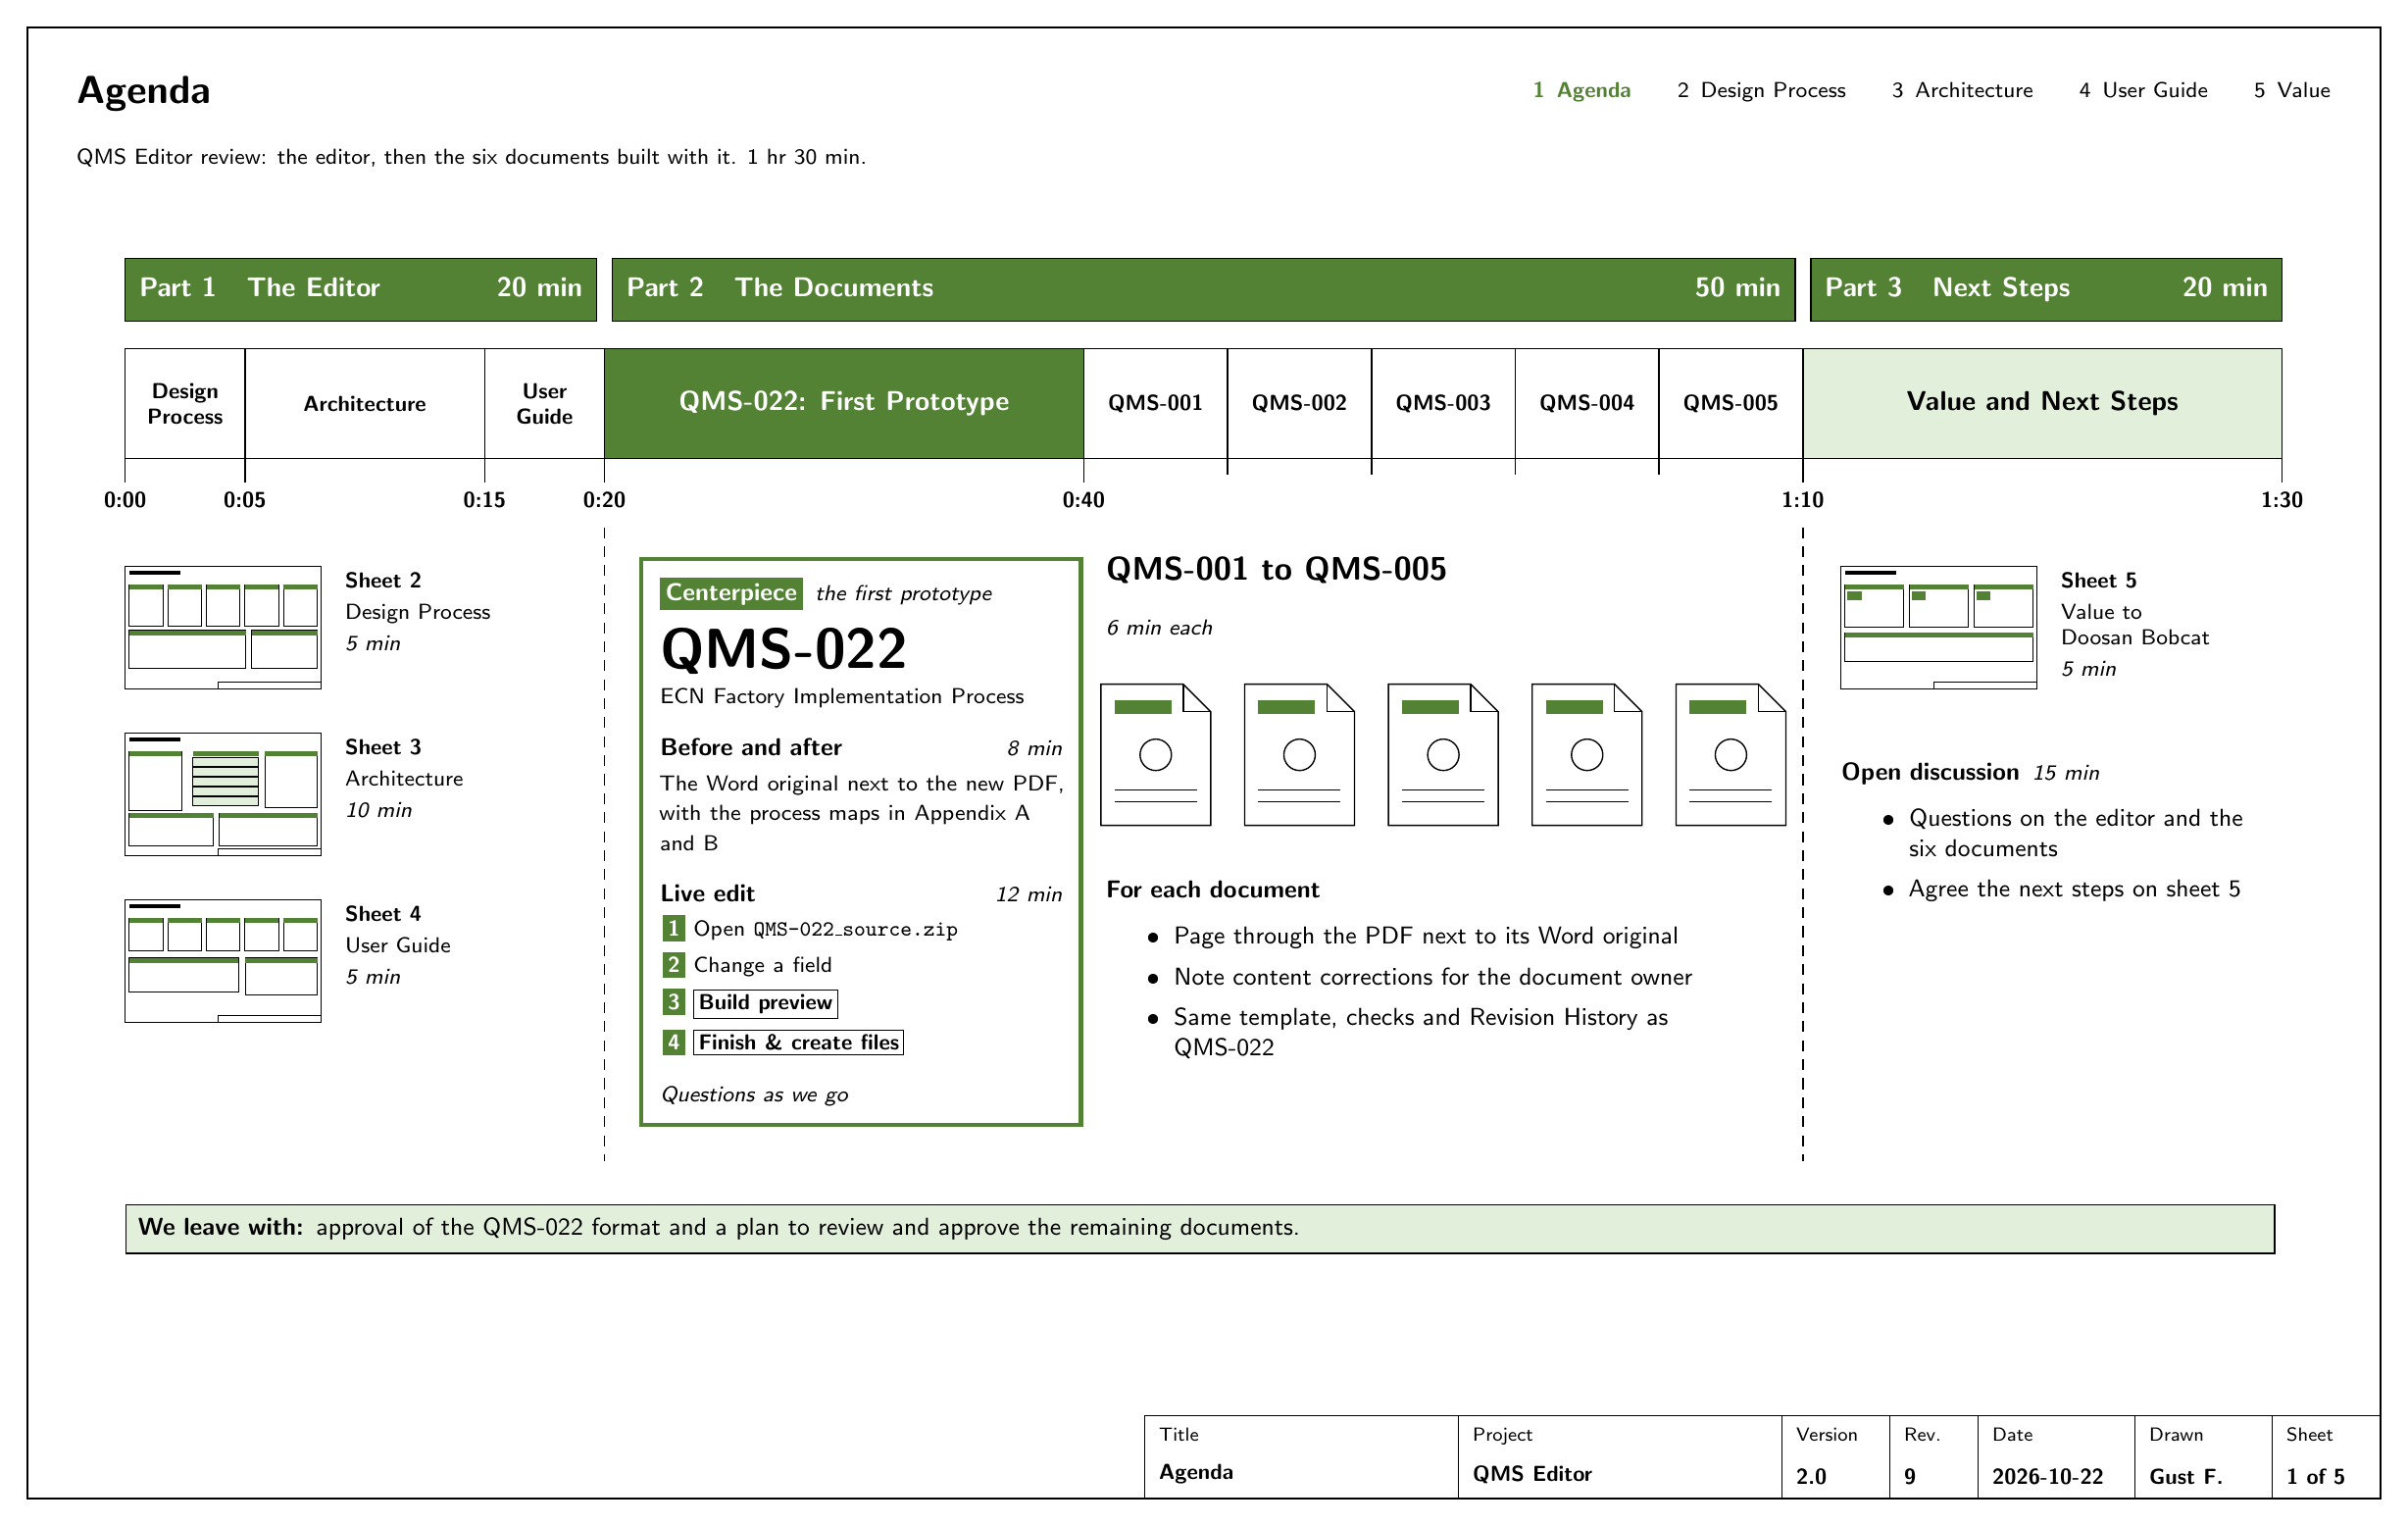
\begin{tikzpicture}[x=1in, y=1in]
\useasboundingbox (0,0) rectangle (12,7.5);
\draw[line width=0.8pt] (0,0) rectangle (12,7.5);
\heading{Agenda}{QMS Editor review: the editor, then the six documents built with it. 1 hr 30 min.}
\nav{1}
% ---- the three parts
\foreach \a/\b/\t/\m in {0.5/2.9044/{Part 1\quad The Editor}/20 min,
                         2.9844/9.0156/{Part 2\quad The Documents}/50 min,
                         9.0956/11.5/{Part 3\quad Next Steps}/20 min} {
  \draw[line width=0.5pt, fill=headgreen] (\a,6.0) rectangle (\b,6.32);
  \node[anchor=west, text=white, font=\sffamily\bfseries\normalsize, text height=1.6ex, text depth=0.45ex] at (\a,6.16) {\t};
  \node[anchor=east, text=white, font=\sffamily\bfseries\normalsize, text height=1.6ex, text depth=0.45ex] at (\b,6.16) {\m};
}
% ---- the timeline, to scale
\foreach \a/\b/\t in {0.5/1.1111/{Design\\Process}, 1.1111/2.3333/{Architecture}, 2.3333/2.9444/{User\\Guide},
                      5.3889/6.1222/{QMS-001}, 6.1222/6.8556/{QMS-002}, 6.8556/7.5889/{QMS-003},
                      7.5889/8.3222/{QMS-004}, 8.3222/9.0556/{QMS-005}} {
  \draw[line width=0.5pt, fill=white] (\a,5.3) rectangle (\b,5.86);
  \node[align=center, font=\sffamily\bfseries\footnotesize, inner sep=0pt] at ({(\a+\b)/2},5.58) {\t};
}
\draw[line width=0.5pt, fill=headgreen] (2.9444,5.3) rectangle (5.3889,5.86);
\node[text=white, font=\sffamily\bfseries\normalsize, inner sep=0pt] at (4.1667,5.58) {QMS-022: First Prototype};
\draw[line width=0.5pt, fill=bandgreen] (9.0556,5.3) rectangle (11.5,5.86);
\node[font=\sffamily\bfseries\normalsize, inner sep=0pt] at (10.2778,5.58) {Value and Next Steps};
\foreach \x/\t in {0.5/0:00, 1.1111/0:05, 2.3333/0:15, 2.9444/0:20, 5.3889/0:40, 9.0556/1:10, 11.5/1:30} {
  \draw[line width=0.5pt] (\x,5.3) -- (\x,5.18);
  \node[anchor=north, font=\sffamily\bfseries\footnotesize, inner sep=0pt] at (\x,5.13) {\t};
}
\foreach \x in {6.1222, 6.8556, 7.5889, 8.3222} \draw[line width=0.5pt] (\x,5.3) -- (\x,5.22);
% ends of parts 1 and 2
\foreach \x in {2.9444, 9.0556} \draw[line width=0.5pt, dash pattern=on 4pt off 3pt] (\x,4.95) -- (\x,1.72);
% ---- part 1: sheets 2 to 4
\foreach \i/\pic/\sheet/\name/\m in {0/\thumbdesign/2/{Design Process}/5 min, 1/\thumbarch/3/{Architecture}/10 min,
                                     2/\thumbguide/4/{User Guide}/5 min} {
  \begin{scope}[shift={(0.5,{4.75-0.85*\i-0.625})}, scale=0.083333, x=1in, y=1in]
    \pic
  \end{scope}
  \node[anchor=north west, align=left, inner sep=0pt, font=\sffamily\footnotesize] at (1.62,{4.72-0.85*\i})
    {\textbf{Sheet \sheet}\\[2pt] \name\\[2pt] {\itshape\m}};
}
% ---- part 2: QMS-022, the centerpiece
\node[anchor=north west, draw=headgreen, line width=1.6pt, fill=white, text width=2.05in, align=left, inner sep=7pt]
  (cp) at (3.12,4.8) {%
  \badge{Centerpiece}\enspace{\footnotesize\itshape the first prototype}\\[6pt]
  {\bfseries\fontsize{20}{22}\selectfont QMS-022}\\[2pt]
  {\footnotesize ECN Factory Implementation Process}\\[8pt]
  \textbf{Before and after}\hfill{\footnotesize\itshape 8 min}\\[2pt]
  {\footnotesize The Word original next to the new PDF, with the process maps in Appendix A and B}\\[8pt]
  \textbf{Live edit}\hfill{\footnotesize\itshape 12 min}\\[3pt]
  {\footnotesize\begin{enumerate}[label=\badge{\arabic*}, leftmargin=1.45em, labelsep=0.35em, itemsep=3pt, topsep=0pt, parsep=0pt]
  \item Open \val{QMS-022\_source.zip}
  \item Change a field
  \item \btn{Build preview}
  \item \btn{Finish \& create files}
  \end{enumerate}}\par\vspace{6pt}
  {\footnotesize\itshape Questions as we go}};
% ---- part 2: QMS-001 to QMS-005
\node[anchor=north west, inner sep=0pt, font=\sffamily\bfseries\large] at (5.5,4.8) {QMS-001 to QMS-005};
\node[anchor=north west, inner sep=0pt, font=\sffamily\footnotesize\itshape] at (5.5,4.48) {6 min each};
\foreach \i in {1,...,5} {
  \pgfmathsetmacro{\xa}{5.3889+(\i-1)*0.7333+0.0867}
  \docicon{\xa}{4.15}
}
\node[anchor=north west, align=left, text width=3.35in, inner sep=0pt] at (5.5,3.15) {\textbf{For each document}\\[3pt]
  \begin{itemize}
  \item Page through the PDF next to its Word original
  \item Note content corrections for the document owner
  \item Same template, checks and Revision History as QMS-022
  \end{itemize}};
% ---- part 3: sheet 5 and the discussion
\begin{scope}[shift={(9.25,{4.75-0.625})}, scale=0.083333, x=1in, y=1in]
  \thumbvalue
\end{scope}
\node[anchor=north west, align=left, inner sep=0pt, font=\sffamily\footnotesize] at (10.37,4.72)
  {\textbf{Sheet 5}\\[2pt] Value to\\Doosan Bobcat\\[2pt] {\itshape 5 min}};
\node[anchor=north west, align=left, text width=2.2in, inner sep=0pt] at (9.25,3.75) {\textbf{Open discussion}\enspace{\footnotesize\itshape 15 min}\\[3pt]
  \begin{itemize}
  \item Questions on the editor and the six documents
  \item Agree the next steps on sheet 5
  \end{itemize}};
% ---- outcome
\node[anchor=north west, draw, line width=0.5pt, fill=bandgreen, text width=10.82in, align=left] at (0.5,1.5)
  {\textbf{We leave with:} approval of the QMS-022 format and a plan to review and approve the remaining documents.};
\titleblock{Agenda}{1 of 5}
\end{tikzpicture}}

\newpage
% ================================================================ sheet 1: design process
% five stations 1.92 in text width (2.06 in overall), 0.3 in arrow gaps, x = 0.25, 2.61, 4.97, 7.33, 9.69
\noindent\scalebox{1.333333}{%
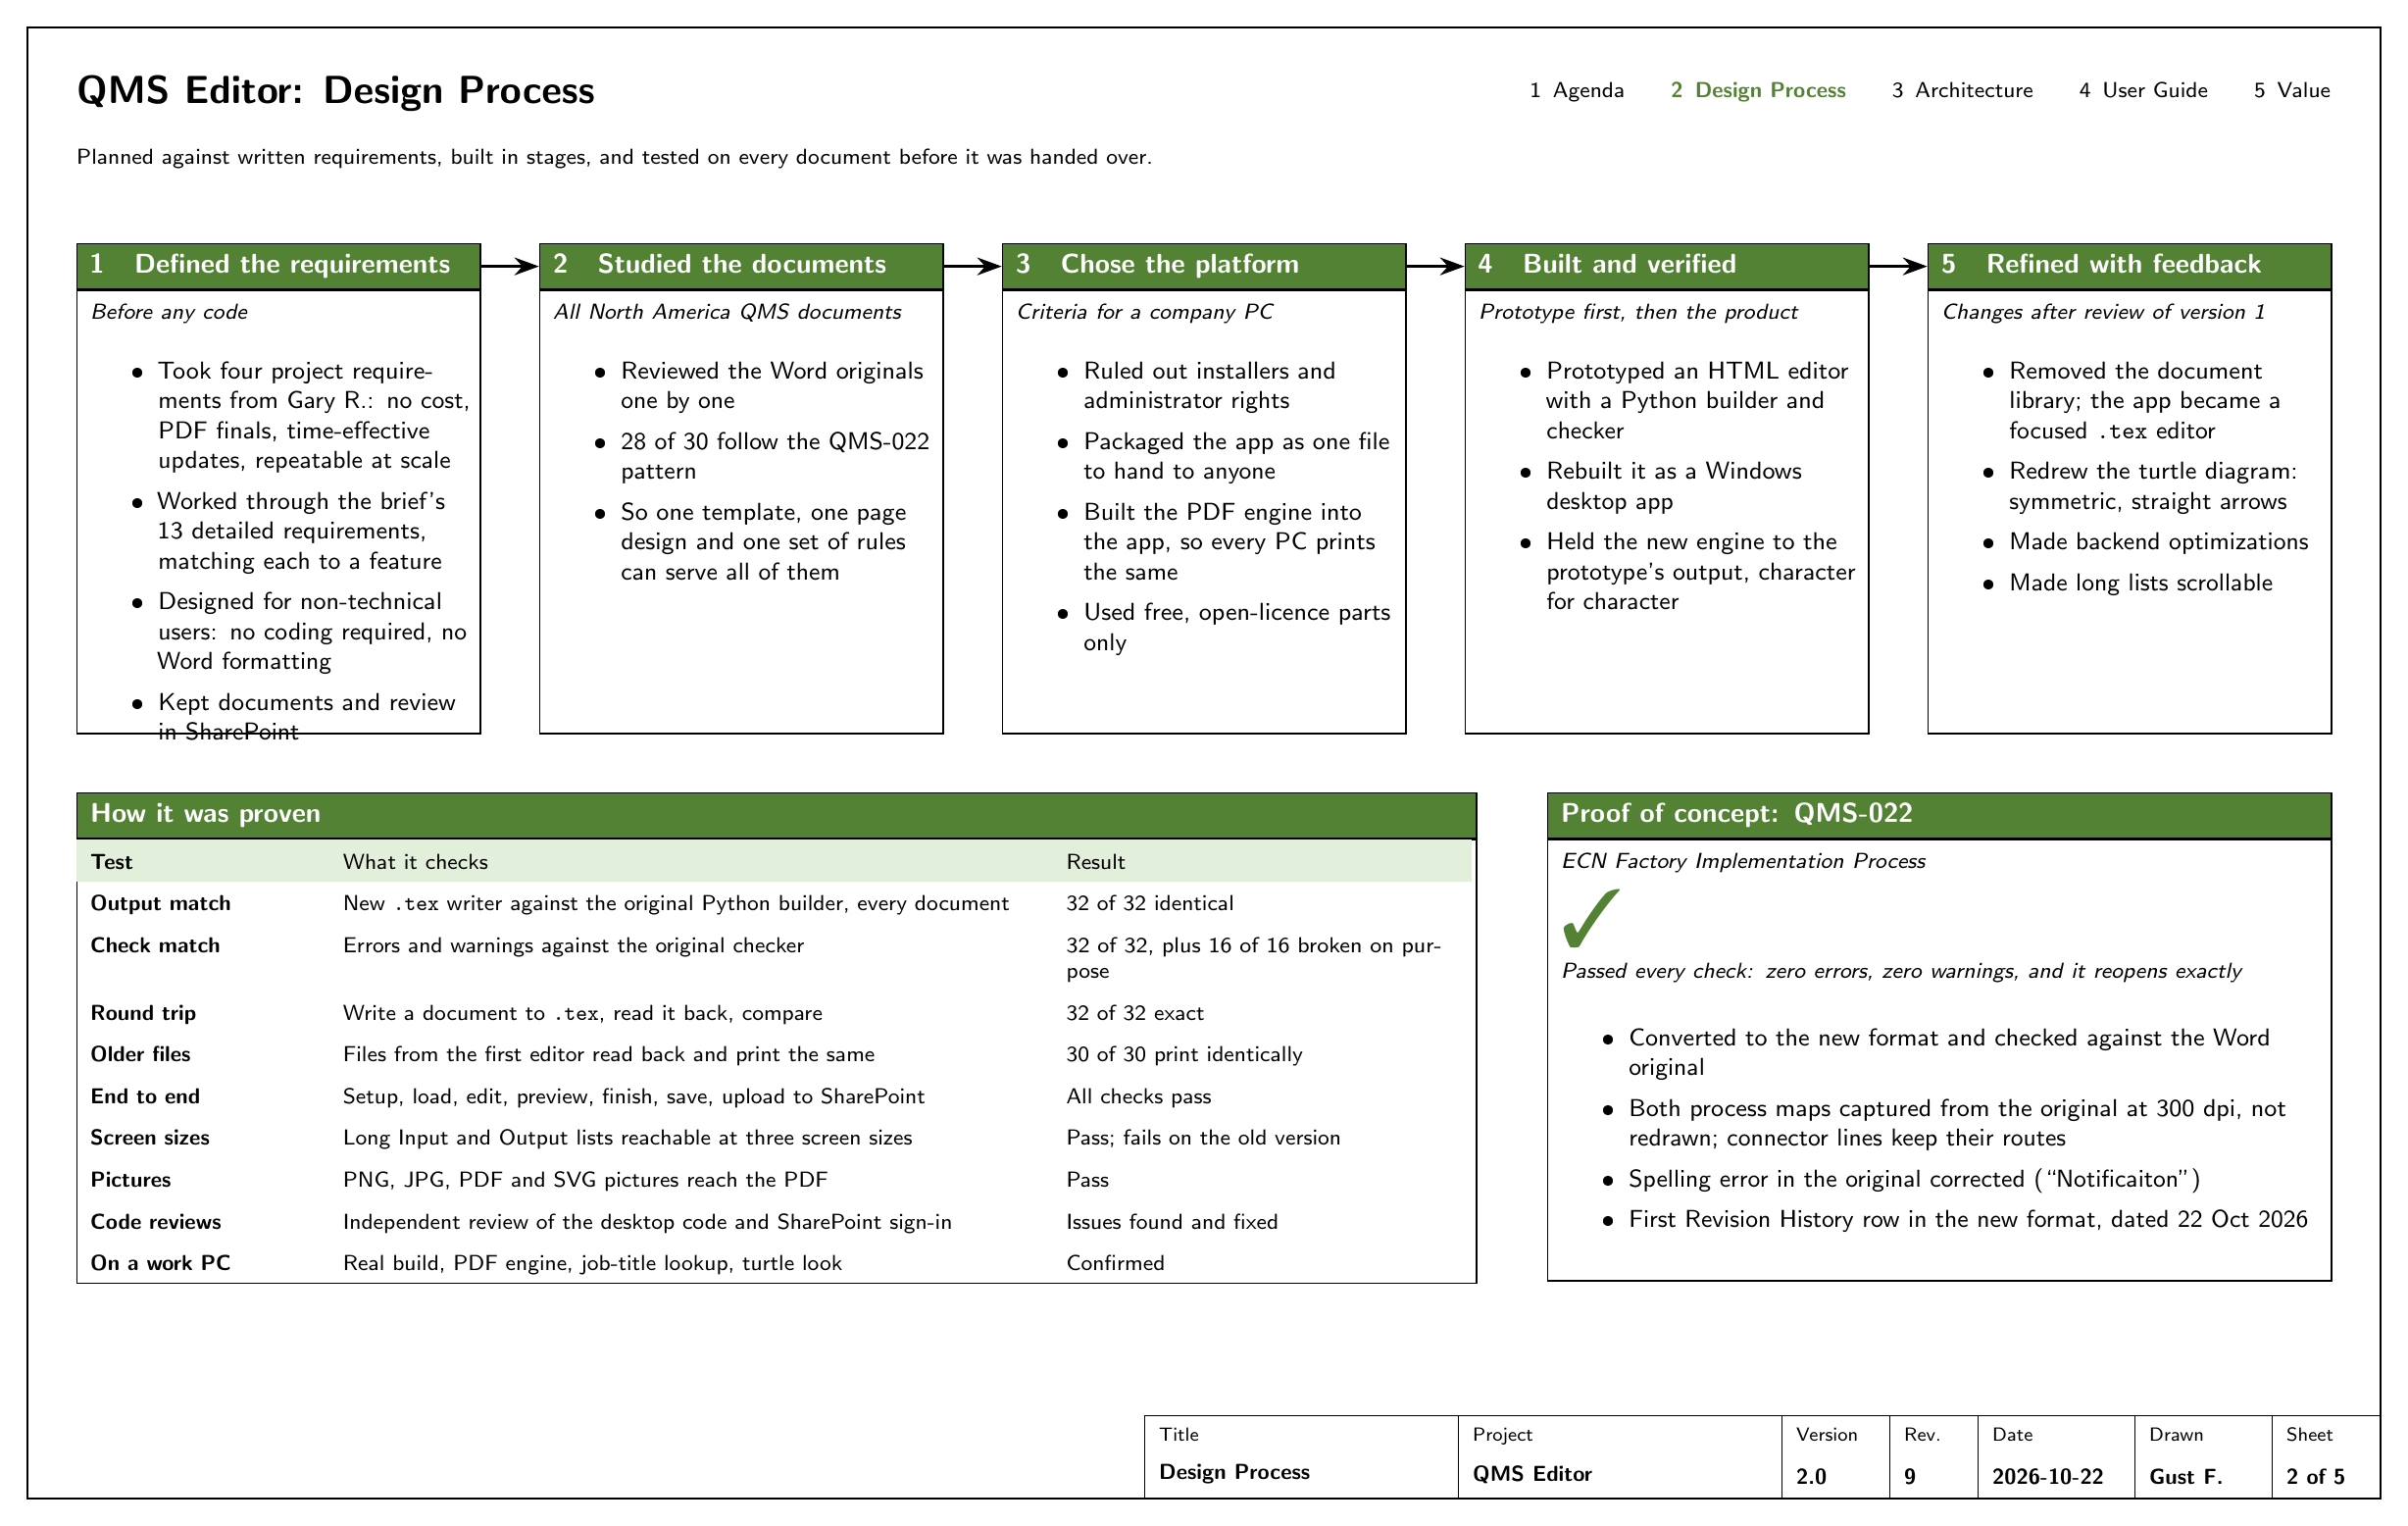
\begin{tikzpicture}[x=1in, y=1in]
\useasboundingbox (0,0) rectangle (12,7.5);
\draw[line width=0.8pt] (0,0) rectangle (12,7.5);
\heading{QMS Editor: Design Process}{Planned against written requirements, built in stages, and tested on
  every document before it was handed over.}
\nav{2}
\node[station, anchor=north west, text width=1.92in] (h1) at (0.25,6.4) {1\quad Defined the requirements};
\node[box, anchor=north, text width=1.92in] (b1) at (h1.south) {\fixh{2.12in}{\by{Before any code}
  \begin{itemize}
  \item Took four project requirements from Gary R.: no cost, PDF finals, time-effective updates, repeatable at scale
  \item Worked through the brief's 13 detailed requirements, matching each to a feature
  \item Designed for non-technical users: no coding required, no Word formatting
  \item Kept documents and review in SharePoint
  \end{itemize}}};
\node[station, anchor=north west, text width=1.92in] (h2) at (2.61,6.4) {2\quad Studied the documents};
\node[box, anchor=north, text width=1.92in] (b2) at (h2.south) {\fixh{2.12in}{\by{All North America QMS documents}
  \begin{itemize}
  \item Reviewed the Word originals one by one
  \item 28 of 30 follow the QMS-022 pattern
  \item So one template, one page design and one set of rules can serve all of them
  \end{itemize}}};
\node[station, anchor=north west, text width=1.92in] (h3) at (4.97,6.4) {3\quad Chose the platform};
\node[box, anchor=north, text width=1.92in] (b3) at (h3.south) {\fixh{2.12in}{\by{Criteria for a company PC}
  \begin{itemize}
  \item Ruled out installers and administrator rights
  \item Packaged the app as one file to hand to anyone
  \item Built the PDF engine into the app, so every PC prints the same
  \item Used free, open-licence parts only
  \end{itemize}}};
\node[station, anchor=north west, text width=1.92in] (h4) at (7.33,6.4) {4\quad Built and verified};
\node[box, anchor=north, text width=1.92in] (b4) at (h4.south) {\fixh{2.12in}{\by{Prototype first, then the product}
  \begin{itemize}
  \item Prototyped an HTML editor with a Python builder and checker
  \item Rebuilt it as a Windows desktop app
  \item Held the new engine to the prototype's output, character for character
  \end{itemize}}};
\node[station, anchor=north west, text width=1.92in] (h5) at (9.69,6.4) {5\quad Refined with feedback};
\node[box, anchor=north, text width=1.92in] (b5) at (h5.south) {\fixh{2.12in}{\by{Changes after review of version 1}
  \begin{itemize}
  \item Removed the document library; the app became a focused \val{.tex} editor
  \item Redrew the turtle diagram: symmetric, straight arrows
  \item Made backend optimizations
  \item Made long lists scrollable
  \end{itemize}}};
\foreach \a/\b in {h1/h2, h2/h3, h3/h4, h4/h5} \draw[flow] (\a.east) -- (\b.west);
% ---- how it was proven
\node[station, anchor=north west, text width=7.0in] (hp) at (0.25,3.6) {How it was proven};
\node[box, anchor=north, inner ysep=0pt, text width=7.0in, font=\sffamily\footnotesize] (bp) at (hp.south) {%
  \setlength{\tabcolsep}{5pt}\renewcommand{\arraystretch}{1.62}%
  \begin{tabular}{@{}>{\bfseries}p{1.15in}p{3.55in}p{2.0in}@{}}
  \rowcolor{bandgreen} Test & What it checks & Result \\
  Output match   & New \val{.tex} writer against the original Python builder, every document & 32 of 32 identical \\
  Check match    & Errors and warnings against the original checker & 32 of 32, plus 16 of 16 broken on purpose \\
  Round trip     & Write a document to \val{.tex}, read it back, compare & 32 of 32 exact \\
  Older files    & Files from the first editor read back and print the same & 30 of 30 print identically \\
  End to end     & Setup, load, edit, preview, finish, save, upload to SharePoint & All checks pass \\
  Screen sizes   & Long Input and Output lists reachable at three screen sizes & Pass; fails on the old version \\
  Pictures       & PNG, JPG, PDF and SVG pictures reach the PDF & Pass \\
  Code reviews   & Independent review of the desktop code and SharePoint sign-in & Issues found and fixed \\
  On a work PC   & Real build, PDF engine, job-title lookup, turtle look & Confirmed \\
  \end{tabular}\par\vspace{5pt}};
% ---- proof of concept
\node[station, anchor=north west, text width=3.86in] (hq) at (7.75,3.6) {Proof of concept: QMS-022};
\node[box, anchor=north, text width=3.86in] (bq) at (hq.south) {\fixh{2.11in}{%
  \by{ECN Factory Implementation Process}
  {\color{headgreen}\fontsize{30}{32}\selectfont\ding{51}}\\[2pt]
  {\footnotesize\itshape Passed every check: zero errors, zero warnings, and it reopens exactly\par}\vspace{8pt}
  \begin{itemize}
  \item Converted to the new format and checked against the Word original
  \item Both process maps captured from the original at 300 dpi, not redrawn; connector lines keep their routes
  \item Spelling error in the original corrected (``Notificaiton'')
  \item First Revision History row in the new format, dated 22 Oct 2026
  \end{itemize}}};
\titleblock{Design Process}{2 of 5}
\end{tikzpicture}}

\newpage
% ================================================================ sheet 2: system architecture
% columns: places 0.25 to 3.45, app 4.15 to 8.15, zip 8.55 to 11.75; lower row from y 2.85
\noindent\scalebox{1.333333}{%
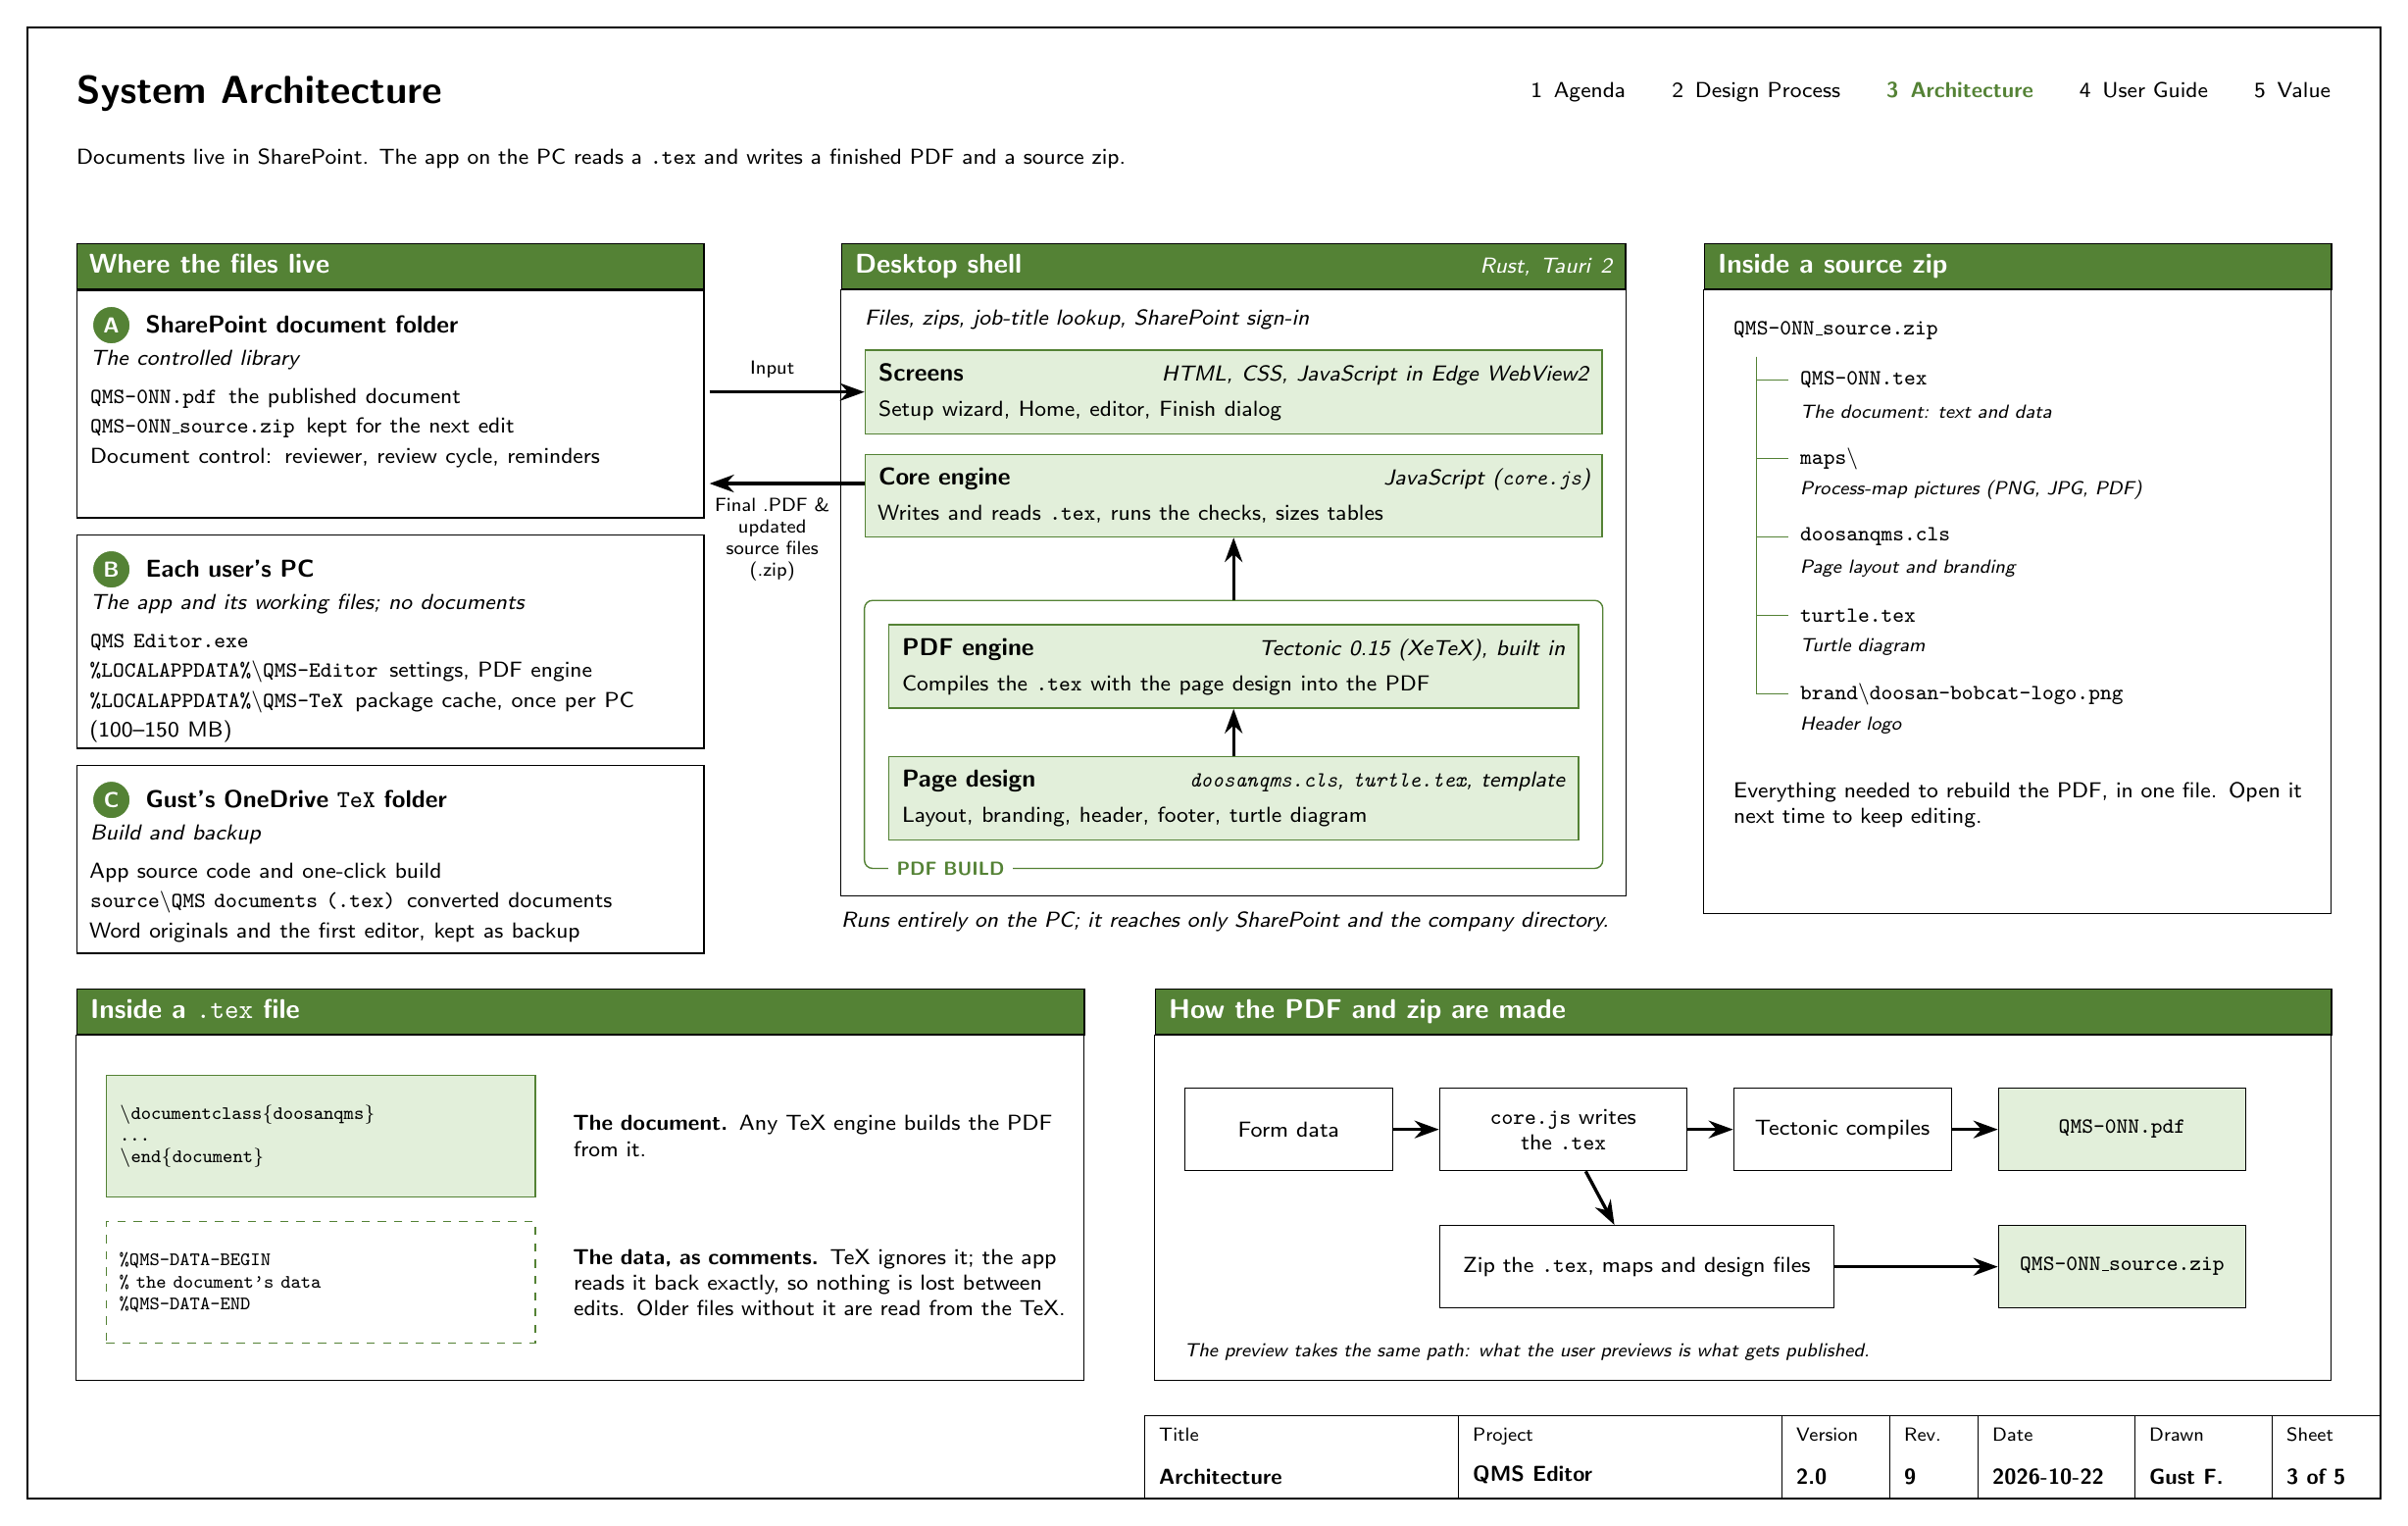
\begin{tikzpicture}[x=1in, y=1in]
\useasboundingbox (0,0) rectangle (12,7.5);
\draw[line width=0.8pt] (0,0) rectangle (12,7.5);
\heading{System Architecture}{Documents live in SharePoint. The app on the PC reads a \val{.tex} and writes a
  finished PDF and a source zip.}
\nav{3}
% ---- where the files live
\node[station, anchor=north west, text width=3.06in] (hw) at (0.25,6.4) {Where the files live};
\node[box, anchor=north, text width=3.06in] (wa) at (hw.south) {\fixh{1.02in}{%
  \textbf{\num{A}\enspace SharePoint document folder}\\[1pt]{\footnotesize\itshape The controlled library}\\[3pt]
  {\footnotesize\val{QMS-0NN.pdf}\enspace the published document\\
  \val{QMS-0NN\_source.zip}\enspace kept for the next edit\\
  Document control: reviewer, review cycle, reminders}}};
\node[box, anchor=north west, text width=3.06in] (wb) at ($(wa.south west)+(0,-0.08)$) {\fixh{0.95in}{%
  \textbf{\num{B}\enspace Each user's PC}\\[1pt]{\footnotesize\itshape The app and its working files; no documents}\\[3pt]
  {\footnotesize\val{QMS Editor.exe}\\
  \val{\%LOCALAPPDATA\%\textbackslash QMS-Editor}\enspace settings, PDF engine\\
  \val{\%LOCALAPPDATA\%\textbackslash QMS-TeX}\enspace package cache, once per PC (100--150 MB)}}};
\node[box, anchor=north west, text width=3.06in] (wc) at ($(wb.south west)+(0,-0.08)$) {\fixh{0.82in}{%
  \textbf{\num{C}\enspace Gust's OneDrive \val{TeX} folder}\\[1pt]{\footnotesize\itshape Build and backup}\\[3pt]
  {\footnotesize App source code and one-click build\\
  \val{source\textbackslash QMS documents (.tex)}\enspace converted documents\\
  Word originals and the first editor, kept as backup}}};
% ---- the desktop shell holds the app: screens, the core engine (which hands the files back to SharePoint),
% ---- and below it the PDF build (page design up into the PDF engine), which flows up into the core engine
\node[station, anchor=north west, text width=3.86in] (ha) at (4.15,6.4)
  {Desktop shell\hfill{\mdseries\footnotesize\itshape Rust, Tauri 2}};
\node[anchor=north west, inner sep=0pt, font=\sffamily\footnotesize\itshape] (cap) at ($(ha.south west)+(0.12,-0.1)$)
  {Files, zips, job-title lookup, SharePoint sign-in};
\node[layer, text width=3.62in] (S) at ($(cap.south west)+(0,-0.1)$)
  {\layerbody{Screens}{HTML, CSS, JavaScript in Edge WebView2}{Setup wizard, Home, editor, Finish dialog}};
\node[layer, text width=3.62in] (CE) at ($(S.south west)+(0,-0.1)$)
  {\layerbody{Core engine}{JavaScript (\val{core.js})}{Writes and reads \val{.tex}, runs the checks, sizes tables}};
\node[layer, text width=3.38in] (PE) at ($(CE.south west)+(0.12,-0.44)$)
  {\layerbody{PDF engine}{Tectonic 0.15 (XeTeX), built in}{Compiles the \val{.tex} with the page design into the PDF}};
\node[layer, text width=3.38in] (PD) at ($(PE.south west)+(0,-0.24)$)
  {\layerbody{Page design}{\val{doosanqms.cls}, \val{turtle.tex}, template}{Layout, branding, header, footer, turtle diagram}};
\draw[line width=0.5pt, draw=headgreen, rounded corners=3pt] ($(CE.south west)+(0,-0.32)$) rectangle ($(PD.south east)+(0.12,-0.14)$);
\node[anchor=west, fill=white, inner xsep=3pt, inner ysep=0pt, text=headgreen, font=\sffamily\bfseries\scriptsize]
  at ($(PD.south west)+(0,-0.14)$) {PDF BUILD};
\draw[line width=0.5pt] (ha.south west) rectangle ($(PD.south east)+(0.24,-0.28)$);
% page design up into the PDF engine, the PDF build up into the core engine: every flow goes up
\draw[flow] (PD.north) -- (PE.south);
\draw[flow] ($(CE.south)+(0,-0.32)$) -- (CE.south);
\node[anchor=north west, inner sep=0pt, text width=4.0in, font=\sffamily\footnotesize] at ($(ha.south west |- PD.south)+(0,-0.36)$)
  {\textit{Runs entirely on the PC; it reaches only SharePoint and the company directory.}};
% in from SharePoint to the screens; out from the core engine straight back to SharePoint.
% Labels centred in the gap between the SharePoint card (right edge 3.45) and the desktop shell (left edge 4.15).
\draw[flow] (3.48,0 |- S.west) -- (S.west);
\node[anchor=south, font=\sffamily\scriptsize, inner sep=0pt] at ($(3.8,0 |- S.west)+(0,0.07)$) {Input};
\coordinate (out) at ($(CE.north west)+(0,-0.15)$);
\draw[flow] (out) -- (3.48,0 |- out);
\node[anchor=north, font=\sffamily\scriptsize, inner sep=0pt, align=center] at ($(3.8,0 |- out)+(0,-0.07)$)
  {Final .PDF \&\\updated\\source files\\(.zip)};
% ---- inside a source zip
\node[station, anchor=north west, text width=3.06in] (hz) at (8.55,6.4) {Inside a source zip};
\draw[line width=0.5pt] (hz.south west) rectangle (11.75,2.98);
\begin{scope}[yshift=0.1in]
\node[anchor=north west, inner sep=0pt, font=\sffamily\bfseries\footnotesize] (zr) at (8.7,5.9) {\val{\bfseries QMS-0NN\_source.zip}};
\foreach \i/\file/\what in {
   1/QMS-0NN.tex/{The document: text and data},
   2/maps\textbackslash/{Process-map pictures (PNG, JPG, PDF)},
   3/doosanqms.cls/{Page layout and branding},
   4/turtle.tex/{Turtle diagram},
   5/brand\textbackslash doosan-bobcat-logo.png/{Header logo}} {
  \draw[line width=0.5pt, headgreen] (8.82,{5.72-(\i-1)*0.4}) -- (8.82,{5.6-(\i-1)*0.4}) -- (8.98,{5.6-(\i-1)*0.4});
  \node[anchor=west, inner sep=0pt, font=\sffamily\footnotesize] at (9.04,{5.6-(\i-1)*0.4}) {\val{\file}};
  \node[anchor=west, inner sep=0pt, font=\sffamily\scriptsize\itshape] at (9.04,{5.44-(\i-1)*0.4}) {\what};
}
\draw[line width=0.5pt, headgreen] (8.82,5.72) -- (8.82,4.0);
\node[anchor=north west, inner sep=0pt, text width=2.9in, font=\sffamily\footnotesize] at (8.7,3.55)
  {Everything needed to rebuild the PDF, in one file. Open it next time to keep editing.};
\end{scope}
% ---- inside a .tex
\node[station, anchor=north west, text width=5.0in] (ht) at (0.25,2.6) {Inside a \val{.tex} file};
\draw[line width=0.5pt] (ht.south west) rectangle (5.39,0.6);
\node[draw=headgreen, line width=0.5pt, fill=bandgreen, anchor=north west, text width=2.05in, minimum height=0.62in,
      font=\ttfamily\scriptsize, align=left] (t1) at (0.4,2.16)
  {\textbackslash documentclass\{doosanqms\}\\ \ldots\\ \textbackslash end\{document\}};
\node[draw=headgreen, line width=0.5pt, dashed, fill=white, anchor=north west, text width=2.05in, minimum height=0.62in,
      font=\ttfamily\scriptsize, align=left] (t2) at ($(t1.south west)+(0,-0.12)$)
  {\%QMS-DATA-BEGIN\\ \% the document's data\\ \%QMS-DATA-END};
\node[anchor=west, text width=2.55in, font=\sffamily\footnotesize, align=left] at ($(t1.east)+(0.12,0)$)
  {\textbf{The document.} Any TeX engine builds the PDF from it.};
\node[anchor=west, text width=2.55in, font=\sffamily\footnotesize, align=left] at ($(t2.east)+(0.12,0)$)
  {\textbf{The data, as comments.} TeX ignores it; the app reads it back exactly, so nothing is lost between edits.
   Older files without it are read from the TeX.};
% ---- how the PDF and zip are made
\node[station, anchor=north west, text width=5.86in] (hm) at (5.75,2.6) {How the PDF and zip are made};
\draw[line width=0.5pt] (hm.south west) rectangle (11.75,0.6);
\node[chip, anchor=west, text width=0.95in] (m1) at (5.9,1.88) {Form data};
\node[chip, anchor=west, text width=1.15in] (m2) at (7.2,1.88) {\val{core.js} writes the \val{.tex}};
\node[chip, anchor=west, text width=1.0in] (m3) at (8.7,1.88) {Tectonic compiles};
\node[outchip, anchor=west, text width=1.15in] (m4) at (10.05,1.88) {\val{\bfseries QMS-0NN.pdf}};
\node[chip, anchor=west, text width=1.9in] (m5) at (7.2,1.18) {Zip the \val{.tex}, maps and design files};
\node[outchip, anchor=west, text width=1.15in] (m6) at (10.05,1.18) {\val{\bfseries QMS-0NN\_source.zip}};
\draw[flow] (m1) -- (m2); \draw[flow] (m2) -- (m3); \draw[flow] (m3) -- (m4);
\draw[flow] (m2) -- (m5); \draw[flow] (m5) -- (m6);
\node[anchor=south west, inner sep=0pt, font=\sffamily\scriptsize\itshape] at (5.9,0.7)
  {The preview takes the same path: what the user previews is what gets published.};
\titleblock{Architecture}{3 of 5}
\end{tikzpicture}}

\newpage
% ================================================================ sheet 3: user guide
\noindent\scalebox{1.333333}{%
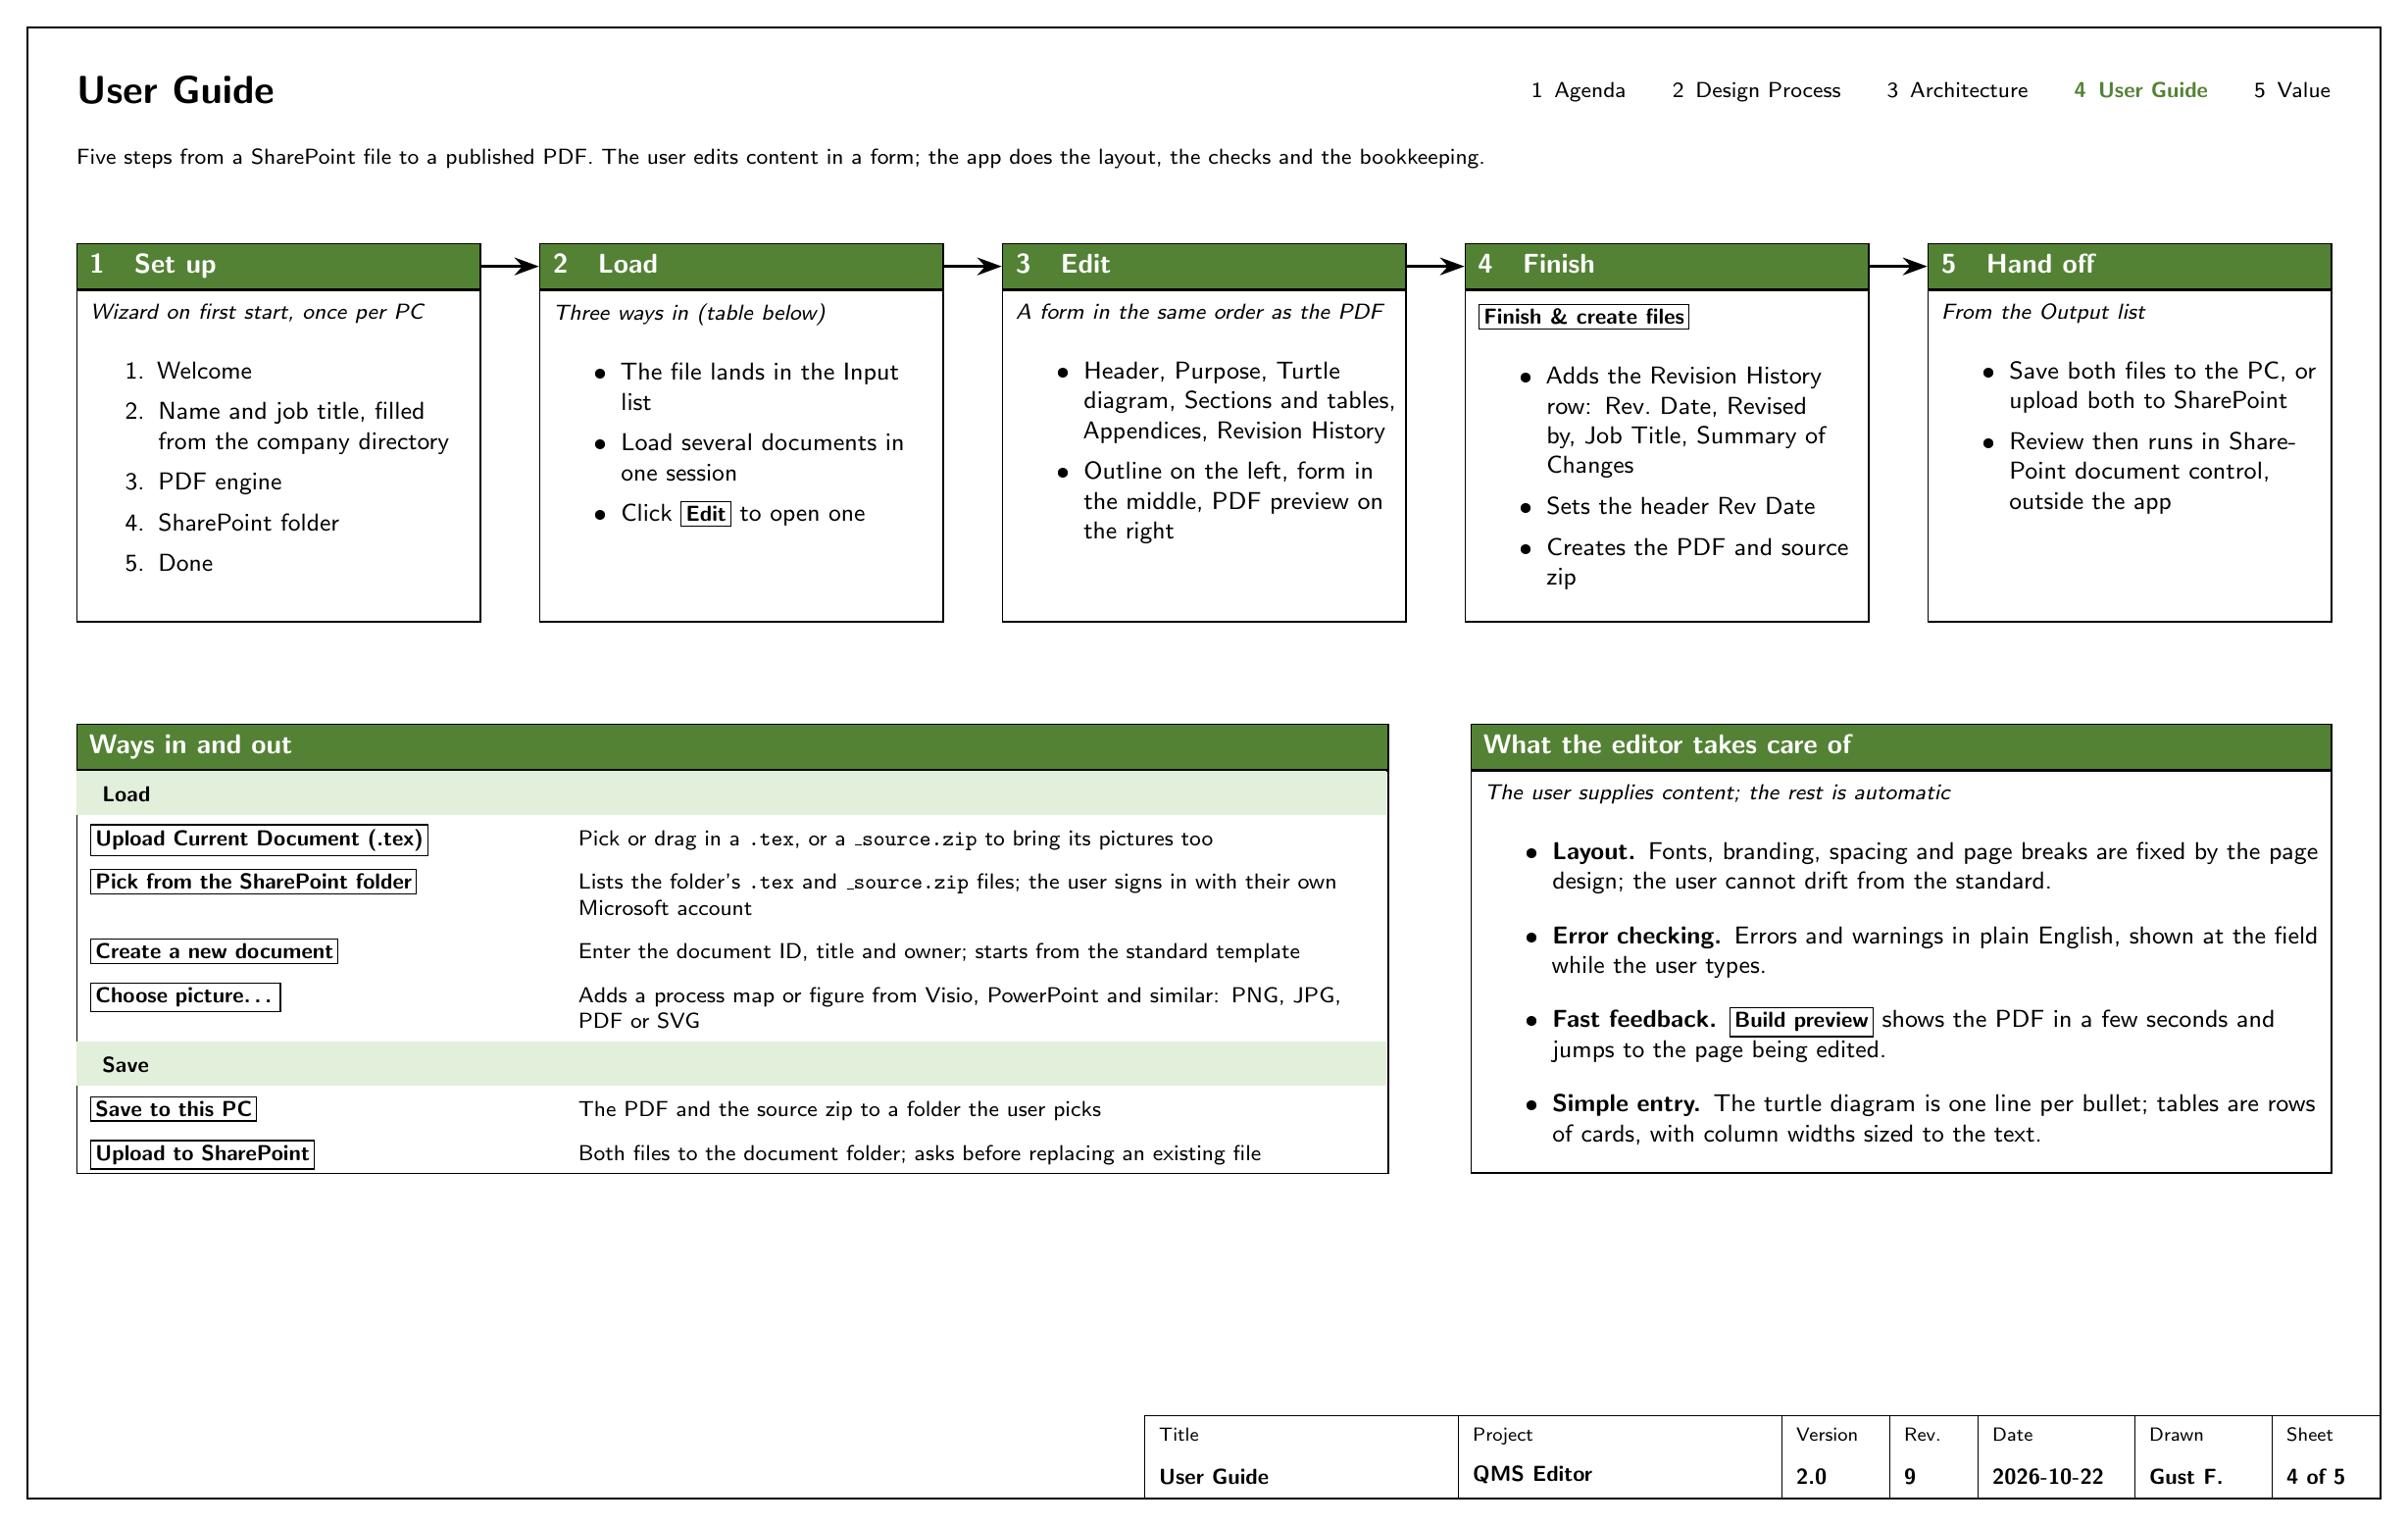
\begin{tikzpicture}[x=1in, y=1in]
\useasboundingbox (0,0) rectangle (12,7.5);
\draw[line width=0.8pt] (0,0) rectangle (12,7.5);
\heading{User Guide}{Five steps from a SharePoint file to a published PDF. The user edits content in a form;
  the app does the layout, the checks and the bookkeeping.}
\nav{4}
\node[station, anchor=north west, text width=1.92in] (h1) at (0.25,6.4) {1\quad Set up};
\node[box, anchor=north, text width=1.92in] (b1) at (h1.south) {\fixh{1.55in}{\by{Wizard on first start, once per PC}
  \begin{enumerate}
  \item Welcome
  \item Name and job title, filled from the company directory
  \item PDF engine
  \item SharePoint folder
  \item Done
  \end{enumerate}}};
\node[station, anchor=north west, text width=1.92in] (h2) at (2.61,6.4) {2\quad Load};
\node[box, anchor=north, text width=1.92in] (b2) at (h2.south) {\fixh{1.55in}{\by{Three ways in (table below)}
  \begin{itemize}
  \item The file lands in the Input list
  \item Load several documents in one session
  \item Click \btn{Edit} to open one
  \end{itemize}}};
\node[station, anchor=north west, text width=1.92in] (h3) at (4.97,6.4) {3\quad Edit};
\node[box, anchor=north, text width=1.92in] (b3) at (h3.south) {\fixh{1.55in}{\by{A form in the same order as the PDF}
  \begin{itemize}
  \item Header, Purpose, Turtle diagram, Sections and tables, Appendices, Revision History
  \item Outline on the left, form in the middle, PDF preview on the right
  \end{itemize}}};
\node[station, anchor=north west, text width=1.92in] (h4) at (7.33,6.4) {4\quad Finish};
\node[box, anchor=north, text width=1.92in] (b4) at (h4.south) {\fixh{1.55in}{\by{\btn{Finish \& create files}}
  \begin{itemize}
  \item Adds the Revision History row: Rev.\ Date, Revised by, Job Title, Summary of Changes
  \item Sets the header Rev Date
  \item Creates the PDF and source zip
  \end{itemize}}};
\node[station, anchor=north west, text width=1.92in] (h5) at (9.69,6.4) {5\quad Hand off};
\node[box, anchor=north, text width=1.92in] (b5) at (h5.south) {\fixh{1.55in}{\by{From the Output list}
  \begin{itemize}
  \item Save both files to the PC, or upload both to SharePoint
  \item Review then runs in SharePoint document control, outside the app
  \end{itemize}}};
\foreach \a/\b in {h1/h2, h2/h3, h3/h4, h4/h5} \draw[flow] (\a.east) -- (\b.west);
% ---- ways in and out
\node[station, anchor=north west, text width=6.55in] (hi) at (0.25,3.95) {Ways in and out};
\node[box, anchor=north, inner ysep=0pt, text width=6.55in, font=\sffamily\footnotesize] (bi) at (hi.south) {%
  \setlength{\tabcolsep}{5pt}\renewcommand{\arraystretch}{1.7}%
  \begin{tabular}{@{}p{2.35in}p{4.05in}@{}}
  \rowcolor{bandgreen}\multicolumn{2}{@{}l@{}}{\bfseries\enspace Load} \\
  \btn{Upload Current Document (.tex)} & Pick or drag in a \val{.tex}, or a \val{\_source.zip} to bring its pictures too \\
  \btn{Pick from the SharePoint folder} & Lists the folder's \val{.tex} and \val{\_source.zip} files; the user signs in with their own Microsoft account \\
  \btn{Create a new document} & Enter the document ID, title and owner; starts from the standard template \\
  \btn{Choose picture\ldots} & Adds a process map or figure from Visio, PowerPoint and similar: PNG, JPG, PDF or SVG \\
  \rowcolor{bandgreen}\multicolumn{2}{@{}l@{}}{\bfseries\enspace Save} \\
  \btn{Save to this PC} & The PDF and the source zip to a folder the user picks \\
  \btn{Upload to SharePoint} & Both files to the document folder; asks before replacing an existing file \\
  \end{tabular}\par\vspace{5pt}};
% ---- what the editor takes care of
\node[station, anchor=north west, text width=4.25in] (he) at (7.36,3.95) {What the editor takes care of};
\node[box, anchor=north, text width=4.25in] (be) at (he.south) {\fixh{1.91in}{%
  \by{The user supplies content; the rest is automatic}
  \begin{itemize}[itemsep=7pt]
  \item \textbf{Layout.} Fonts, branding, spacing and page breaks are fixed by the page design; the user cannot drift from the standard.
  \item \textbf{Error checking.} Errors and warnings in plain English, shown at the field while the user types.
  \item \textbf{Fast feedback.} \btn{Build preview} shows the PDF in a few seconds and jumps to the page being edited.
  \item \textbf{Simple entry.} The turtle diagram is one line per bullet; tables are rows of cards, with column widths sized to the text.
  \end{itemize}}};
\titleblock{User Guide}{4 of 5}
\end{tikzpicture}}

\newpage
% ================================================================ sheet 4: value to Doosan Bobcat
% three stations 3.46 in text width (3.6 in overall), 0.35 in gaps, x = 0.25, 4.2, 8.15
\noindent\scalebox{1.333333}{%
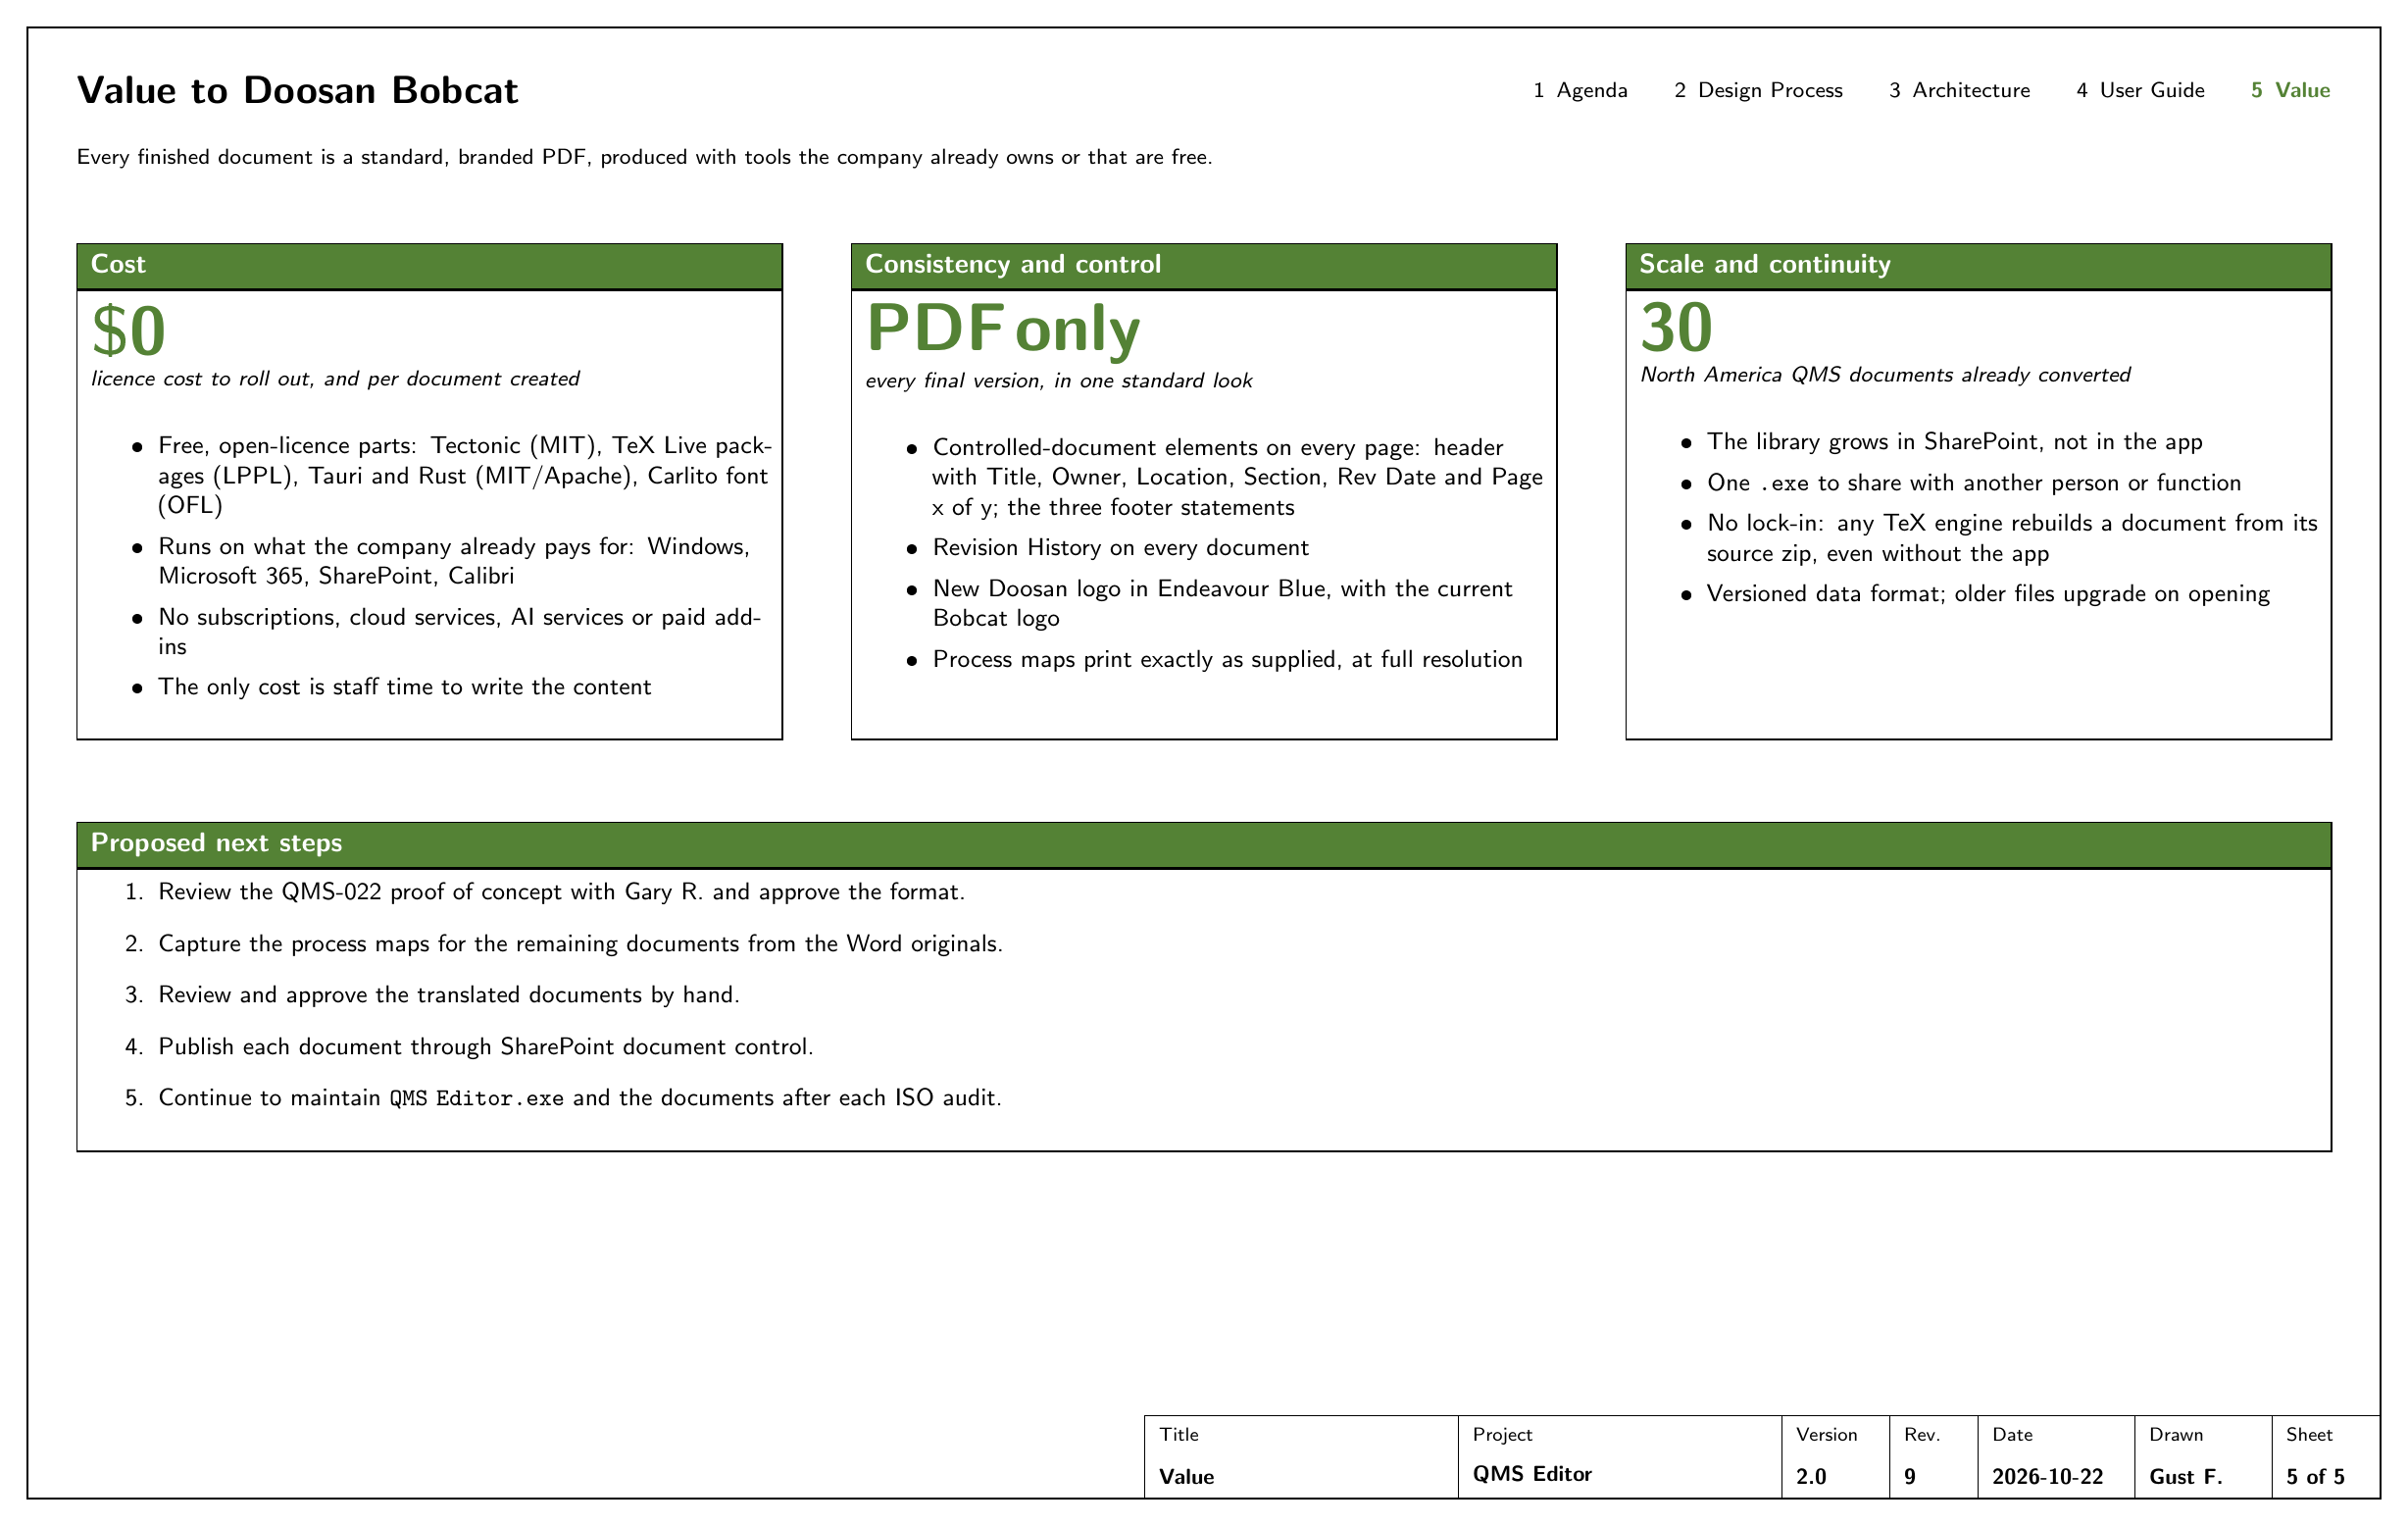
\begin{tikzpicture}[x=1in, y=1in]
\useasboundingbox (0,0) rectangle (12,7.5);
\draw[line width=0.8pt] (0,0) rectangle (12,7.5);
\heading{Value to Doosan Bobcat}{Every finished document is a standard, branded PDF, produced with tools the
  company already owns or that are free.}
\nav{5}
\node[station, anchor=north west, text width=3.46in] (h1) at (0.25,6.4) {Cost};
\node[box, anchor=north, text width=3.46in] (b1) at (h1.south) {\fixh{2.15in}{%
  \stat{\$0}{licence cost to roll out, and per document created}
  \begin{itemize}
  \item Free, open-licence parts: Tectonic (MIT), TeX Live packages (LPPL), Tauri and Rust (MIT/Apache), Carlito font (OFL)
  \item Runs on what the company already pays for: Windows, Microsoft~365, SharePoint, Calibri
  \item No subscriptions, cloud services, AI services or paid add-ins
  \item The only cost is staff time to write the content
  \end{itemize}}};
\node[station, anchor=north west, text width=3.46in] (h2) at (4.2,6.4) {Consistency and control};
\node[box, anchor=north, text width=3.46in] (b2) at (h2.south) {\fixh{2.15in}{%
  \stat{PDF only}{every final version, in one standard look}
  \begin{itemize}
  \item Controlled-document elements on every page: header with Title, Owner, Location, Section, Rev Date and Page x of y; the three footer statements
  \item Revision History on every document
  \item New Doosan logo in Endeavour Blue, with the current Bobcat logo
  \item Process maps print exactly as supplied, at full resolution
  \end{itemize}}};
\node[station, anchor=north west, text width=3.46in] (h3) at (8.15,6.4) {Scale and continuity};
\node[box, anchor=north, text width=3.46in] (b3) at (h3.south) {\fixh{2.15in}{%
  \stat{30}{North America QMS documents already converted}
  \begin{itemize}
  \item The library grows in SharePoint, not in the app
  \item One \val{.exe} to share with another person or function
  \item No lock-in: any TeX engine rebuilds a document from its source zip, even without the app
  \item Versioned data format; older files upgrade on opening
  \end{itemize}}};
% ---- next steps
\node[station, anchor=north west, text width=11.36in] (hn) at (0.25,3.45) {Proposed next steps};
\node[box, anchor=north, text width=11.36in] (bn) at (hn.south) {\fixh{1.3in}{%
  \begin{enumerate}[itemsep=6pt]
  \item Review the QMS-022 proof of concept with Gary R. and approve the format.
  \item Capture the process maps for the remaining documents from the Word originals.
  \item Review and approve the translated documents by hand.
  \item Publish each document through SharePoint document control.
  \item Continue to maintain \val{QMS Editor.exe} and the documents after each ISO audit.
  \end{enumerate}}};
\titleblock{Value}{5 of 5}
\end{tikzpicture}}
\end{document}
